\documentclass [tikz] {standalone}

\input{header.htex}

\begin {document}

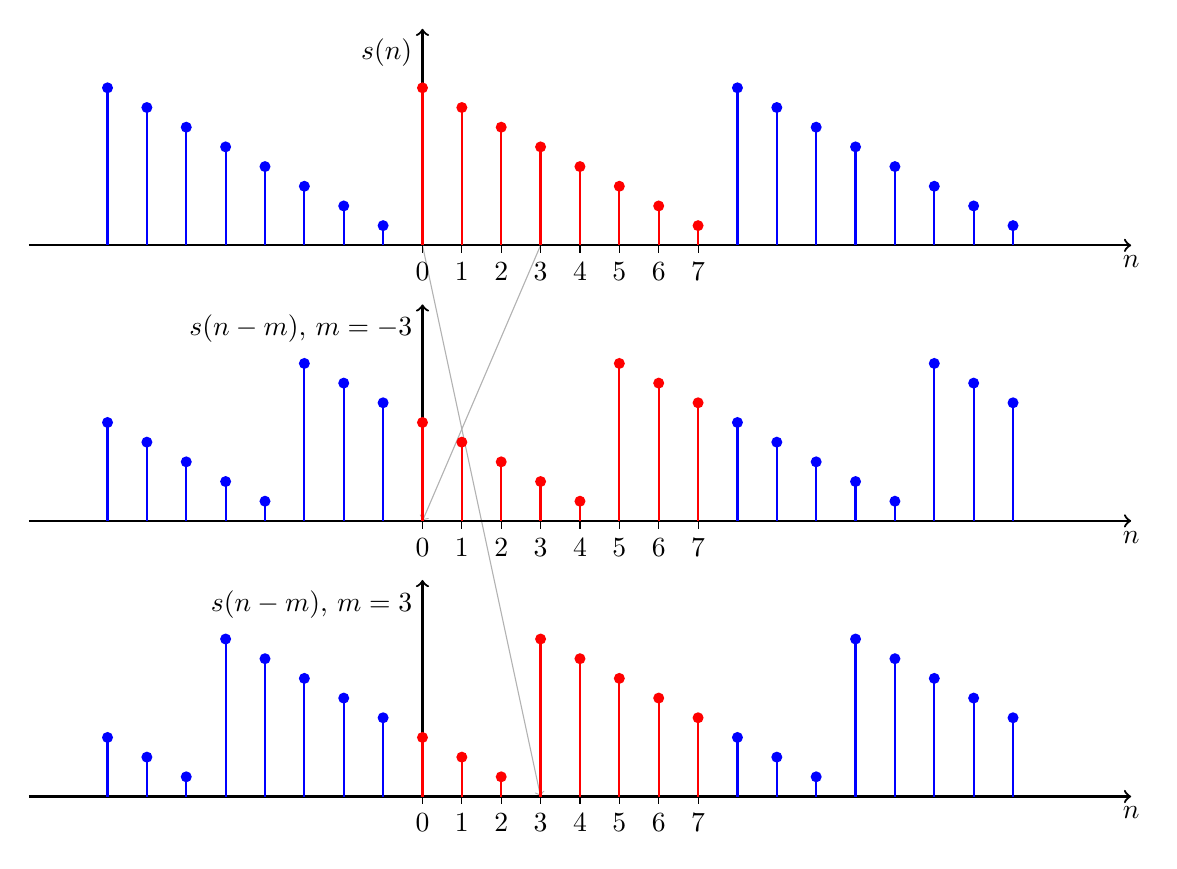
\begin{tikzpicture}

%\\filldraw[fill=yellow!20!white, draw=yellow] (-0.2,2.5) rectangle (0.2,-0.2);

\draw[->,thick] (-5cm,	0cm)		-- (9cm, 0cm)	node[below] {$n$};
\draw[->,thick] ( 0cm,	0cm)		-- (   0cm, 2.75cm)	node[below left] {$s(n)$};

\draw[->, draw=white!70!black] (1.5,0) -- (0,-3.5);
\draw[->, draw=white!70!black] (0,0) -- (1.5,-7);


\begin{scope}[blue]
\foreach \z in {0, 1, ..., 7}
{	
	\draw [thick] (\z * 0.5 - 4, 0cm) -- (\z * 0.5 - 4, 2.0 - \z*0.25);
	\fill (\z * 0.5 - 4, 2.0 - \z*0.25 ) circle(0.07cm);
	
	\draw [thick] (\z * 0.5 + 4, 0cm) -- (\z * 0.5 + 4, 2.0 - \z*0.25);
	\fill (\z * 0.5 + 4, 2.0 - \z*0.25 ) circle(0.07cm);
}
\end{scope}

\begin{scope}[red]
\foreach \z in {0, 1, ..., 7}
{	
	\draw [thick] (\z * 0.5 - 0, 0cm) -- (\z * 0.5 - 0, 2.0 - \z*0.25);
	\fill (\z * 0.5 - 0, 2.0 - \z*0.25 ) circle(0.07cm);

}
\end{scope}

\foreach \z in {0, 1, ..., 7}
{	
	\draw [thin] (\z * 0.5 - 0, 0cm) -- (\z * 0.5 - 0, -0.1) node[below] {$\z$};
}


\draw[->,thick] (-5cm,	-3.5cm)		-- (9cm, -3.5cm)	node[below] {$n$};
\draw[->,thick] ( 0cm,	-3.5cm)		-- (0cm, -0.75cm)	node[below left] {$s(n-m)$, $m = -3$};

\begin{scope}[blue]
\foreach \z in {0, 1, ..., 4}
{	
	\draw [thick] (\z * 0.5 - 4, -3.5cm) -- (\z * 0.5 - 4, 2.0 - \z*0.25 - 3*0.25 - 3.5);
	\fill (\z * 0.5 - 4, 2.0 - \z*0.25- 3*0.25 - 3.5 ) circle(0.07cm);
	
	\draw [thick] (\z * 0.5 + 4, -3.5cm) -- (\z * 0.5 + 4, 2.0 - \z*0.25 - 3*0.25 - 3.5);
	\fill (\z * 0.5 + 4, 2.0 - \z*0.25- 3*0.25 - 3.5 ) circle(0.07cm);
}
\foreach \z in {0, 1, ..., 2}
{	
	\draw [thick] (\z * 0.5 - 1.5, -3.5cm) -- (\z * 0.5 - 1.5, 2.0 - \z*0.25  - 3.5);
	\fill (\z * 0.5 - 1.5, 2.0 - \z*0.25  - 3.5) circle(0.07cm);
	
	\draw [thick] (\z * 0.5 + 6.5, -3.5cm) -- (\z * 0.5 + 6.5, 2.0 - \z*0.25  - 3.5);
	\fill (\z * 0.5 + 6.5, 2.0 - \z*0.25  - 3.5) circle(0.07cm);
}
\end{scope}

\begin{scope}[red]
\foreach \z in {0, 1, ..., 4}
{	
	\draw [thick] (\z * 0.5 - 0, -3.5cm) -- (\z * 0.5 - 0, 2.0 - \z*0.25 - 3*0.25 - 3.5);
	\fill (\z * 0.5 - 0, 2.0 - \z*0.25 - 3*0.25 - 3.5) circle(0.07cm);
	
}
\foreach \z in {0, 1, ..., 2}
{	
	\draw [thick] (\z * 0.5 +2.5, -3.5cm) -- (\z * 0.5 +2.5, 2.0 - \z*0.25  - 3.5);
	\fill (\z * 0.5 +2.5, 2.0 - \z*0.25  - 3.5) circle(0.07cm);
}
\end{scope}

\foreach \z in {0, 1, ..., 7}
{	
	\draw [thin] (\z * 0.5 - 0, -3.5cm) -- (\z * 0.5 - 0, -3.6) node[below] {$\z$};
}




\draw[->,thick] (-5cm,	-7cm)		-- (9cm, -7cm)	node[below] {$n$};
\draw[->,thick] ( 0cm,	-7cm)		-- (0cm, -4.25cm)	node[below left] {$s(n-m)$, $m = 3$};


\begin{scope}[blue]
\foreach \z in {0, 1, ..., 2}
{	
	\draw [thick] (\z * 0.5 - 4, -7cm) -- (\z * 0.5 - 4, 2.0 - \z*0.25 - 5*0.25  - 7);
	\fill (\z * 0.5 - 4, 2.0 - \z*0.25 - 5*0.25  - 7) circle(0.07cm);
	
	\draw [thick] (\z * 0.5 + 4, -7cm) -- (\z * 0.5 + 4, 2.0 - \z*0.25 - 5*0.25  - 7);
	\fill (\z * 0.5 + 4, 2.0 - \z*0.25 - 5*0.25  - 7) circle(0.07cm);
}


\foreach \z in {0, 1, ..., 4}
{	
	\draw [thick] (\z * 0.5 - 2.5, -7cm) -- (\z * 0.5 - 2.5, 2.0 - \z*0.25  - 7);
	\fill (\z * 0.5 - 2.5, 2.0 - \z*0.25  - 7 ) circle(0.07cm);
	
	\draw [thick] (\z * 0.5 + 5.5, -7cm) -- (\z * 0.5 + 5.5, 2.0 - \z*0.25  - 7);
	\fill (\z * 0.5 + 5.5, 2.0 - \z*0.25  - 7 ) circle(0.07cm);
}


\end{scope}


\begin{scope}[red]
\foreach \z in {0, 1, ..., 2}
{	
	\draw [thick] (\z * 0.5, -7cm) -- (\z * 0.5, 2.0 - \z*0.25 - 5*0.25  - 7);
	\fill (\z * 0.5, 2.0 - \z*0.25 - 5*0.25  - 7) circle(0.07cm);
	

}


\foreach \z in {0, 1, ..., 4}
{	
	\draw [thick] (\z * 0.5 + 1.5, -7cm) -- (\z * 0.5 +1.5, 2.0 - \z*0.25  - 7);
	\fill (\z * 0.5 +1.5, 2.0 - \z*0.25  - 7 ) circle(0.07cm);
	

}
\end{scope}



\foreach \z in {0, 1, ..., 7}
{	
	\draw [thin] (\z * 0.5 - 0, -7cm) -- (\z * 0.5 - 0, -7.1) node[below] {$\z$};
}






\end{tikzpicture}
\end {document}
%		\caption{Пример циклического сдвига сигнала}\label{dftprop:fig1}
%	\end{center}
%\end{figure}
